\chapter{Design and Architecture}
\label{ch:architecture}

This chapter translates the requirements and sprint plan of Chapter~\ref{ch:requirements}
into a concrete system design. The presentation follows two complementary views:
\begin{itemize}[leftmargin=*,itemsep=0.2em]
  \item \textbf{Static design} (Sections~\ref{sec:overall-architecture}--\ref{sec:technology-justification}) --- platform architecture, subsystem responsibilities, persisted domain model, and technology justification;
  \item \textbf{Dynamic design} (Section~\ref{sec:sprint-design}) --- sprint-scoped use-case and class models, followed by interaction sequence diagrams for every major API and UX flow.
\end{itemize}
Implementation details and validation evidence are developed in
Chapters~\ref{ch:implementation} and~\ref{ch:validation}.

\section{Overall Solution Architecture}
\label{sec:overall-architecture}

The Knowledge Platform follows a three-tier logical architecture: browser client, API layer, and data/AI services. Figure~\ref{fig:architecture} summarizes component responsibilities and data flows (see also Appendix~\ref{fig:annex-architecture} for the full exported diagram).

\begin{figure}[H]
\centering
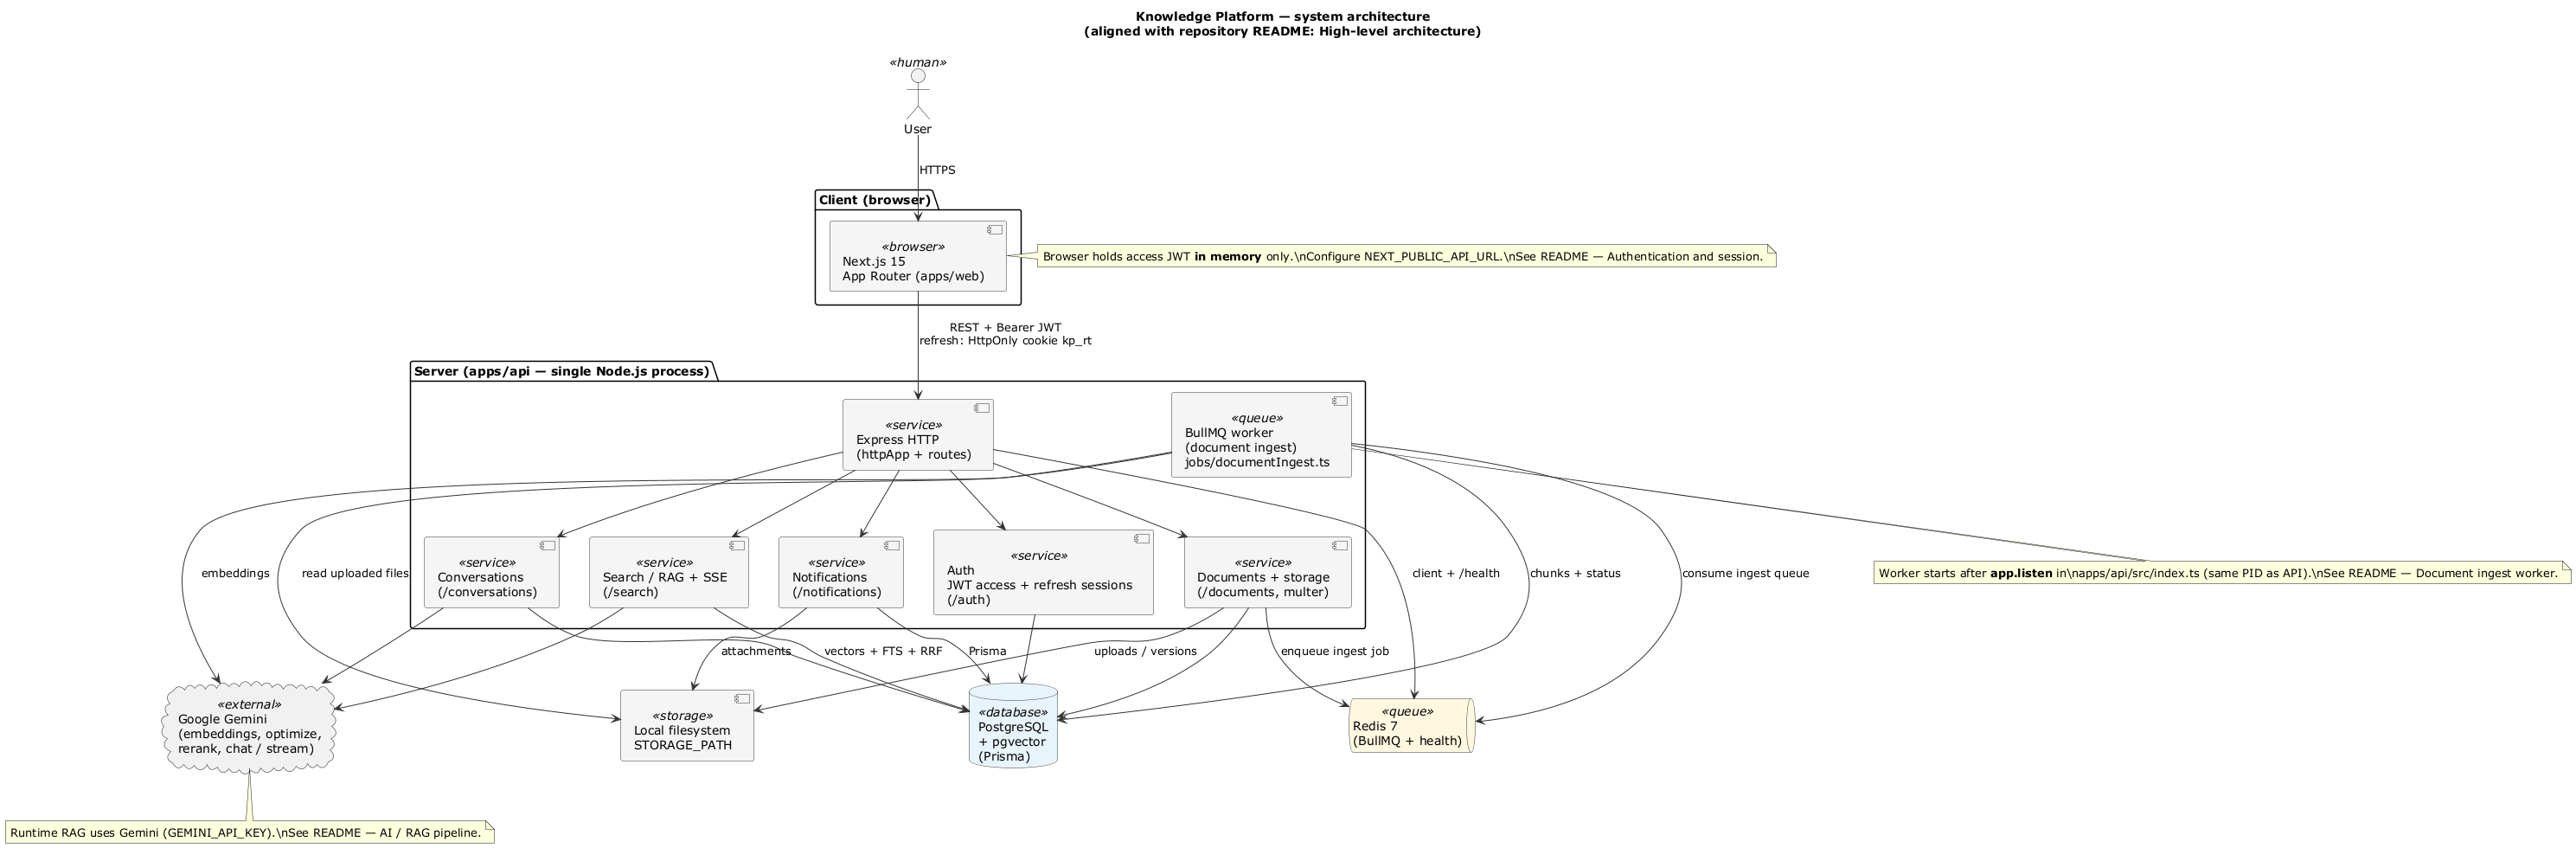
\includegraphics[width=0.98\textwidth]{assets/figures/platform-architecture.png}
\caption[Overall platform architecture]{Overall architecture of the Knowledge Platform (PlantUML source: \texttt{platform-architecture.puml})}
\label{fig:architecture}
\end{figure}

The web application (\texttt{apps/web}) keeps access tokens in memory and uses HttpOnly refresh cookies. The API (\texttt{apps/api}) mounts routers for \texttt{/auth}, \texttt{/documents}, \texttt{/search}, \texttt{/conversations}, \texttt{/admin}, \texttt{/manager}, \texttt{/notifications}, and public \texttt{/avatars}. A BullMQ consumer runs in the same Node process after the HTTP server starts.

\section{Logical Subsystem Decomposition}
\label{sec:subsystem-decomposition}

\begin{table}[H]
\centering
\caption{Subsystem responsibilities}
\label{tab:subsystems}
\renewcommand{\arraystretch}{1.35}
\begin{tabularx}{\textwidth}{|>{\RaggedRight\arraybackslash}p{2.5cm}|Y|>{\RaggedRight\arraybackslash}p{3.1cm}|}
\hline
\rowcolor{sectionblue!15}
\textbf{Subsystem} & \textbf{Responsibility} & \textbf{Key modules} \\
\hline
Authentication & Login, refresh families, restrictions, password reset &
\tcodelines{auth.ts}{authClient.ts} \\
\hline
Documents & CRUD, versions, visibility, audit, download &
\tcodelines{documents.ts}{storage.ts} \\
\hline
Ingest worker & Extract, chunk, embed, persist chunks &
\tcodelines{BullMQ worker}{index.ts} \\
\hline
Search / RAG & Hybrid retrieval, SSE answers, cache &
\tcodelines{search.ts}{ragCompletion.ts} \\
\hline
Conversations & Threads, messages, feedback &
\tcode{conversations.ts} \\
\hline
Notifications & Auto events and manual announcements &
\tcode{notifications.ts} \\
\hline
Admin / Manager & Governance dashboards &
\tcodelines{admin.ts}{manager.ts} \\
\hline
\end{tabularx}
\end{table}

\section{Domain Data Model}
\label{sec:domain-model}

The Prisma schema defines 20+ entities including \texttt{User}, \texttt{Department},
\texttt{Document}, \texttt{DocumentVersion}, \texttt{Chunk} (768-d embedding),
\texttt{Conversation}, \texttt{AnswerFeedback}, and \texttt{Notification}.
Multi-department access is modeled through \texttt{UserDepartmentAccess}.
Figure~\ref{fig:class-diagram} presents the principal persisted classes and their
relationships across all sprints; sprint-scoped excerpts appear in
Section~\ref{sec:sprint-design}.

\begin{figure}[H]
\centering
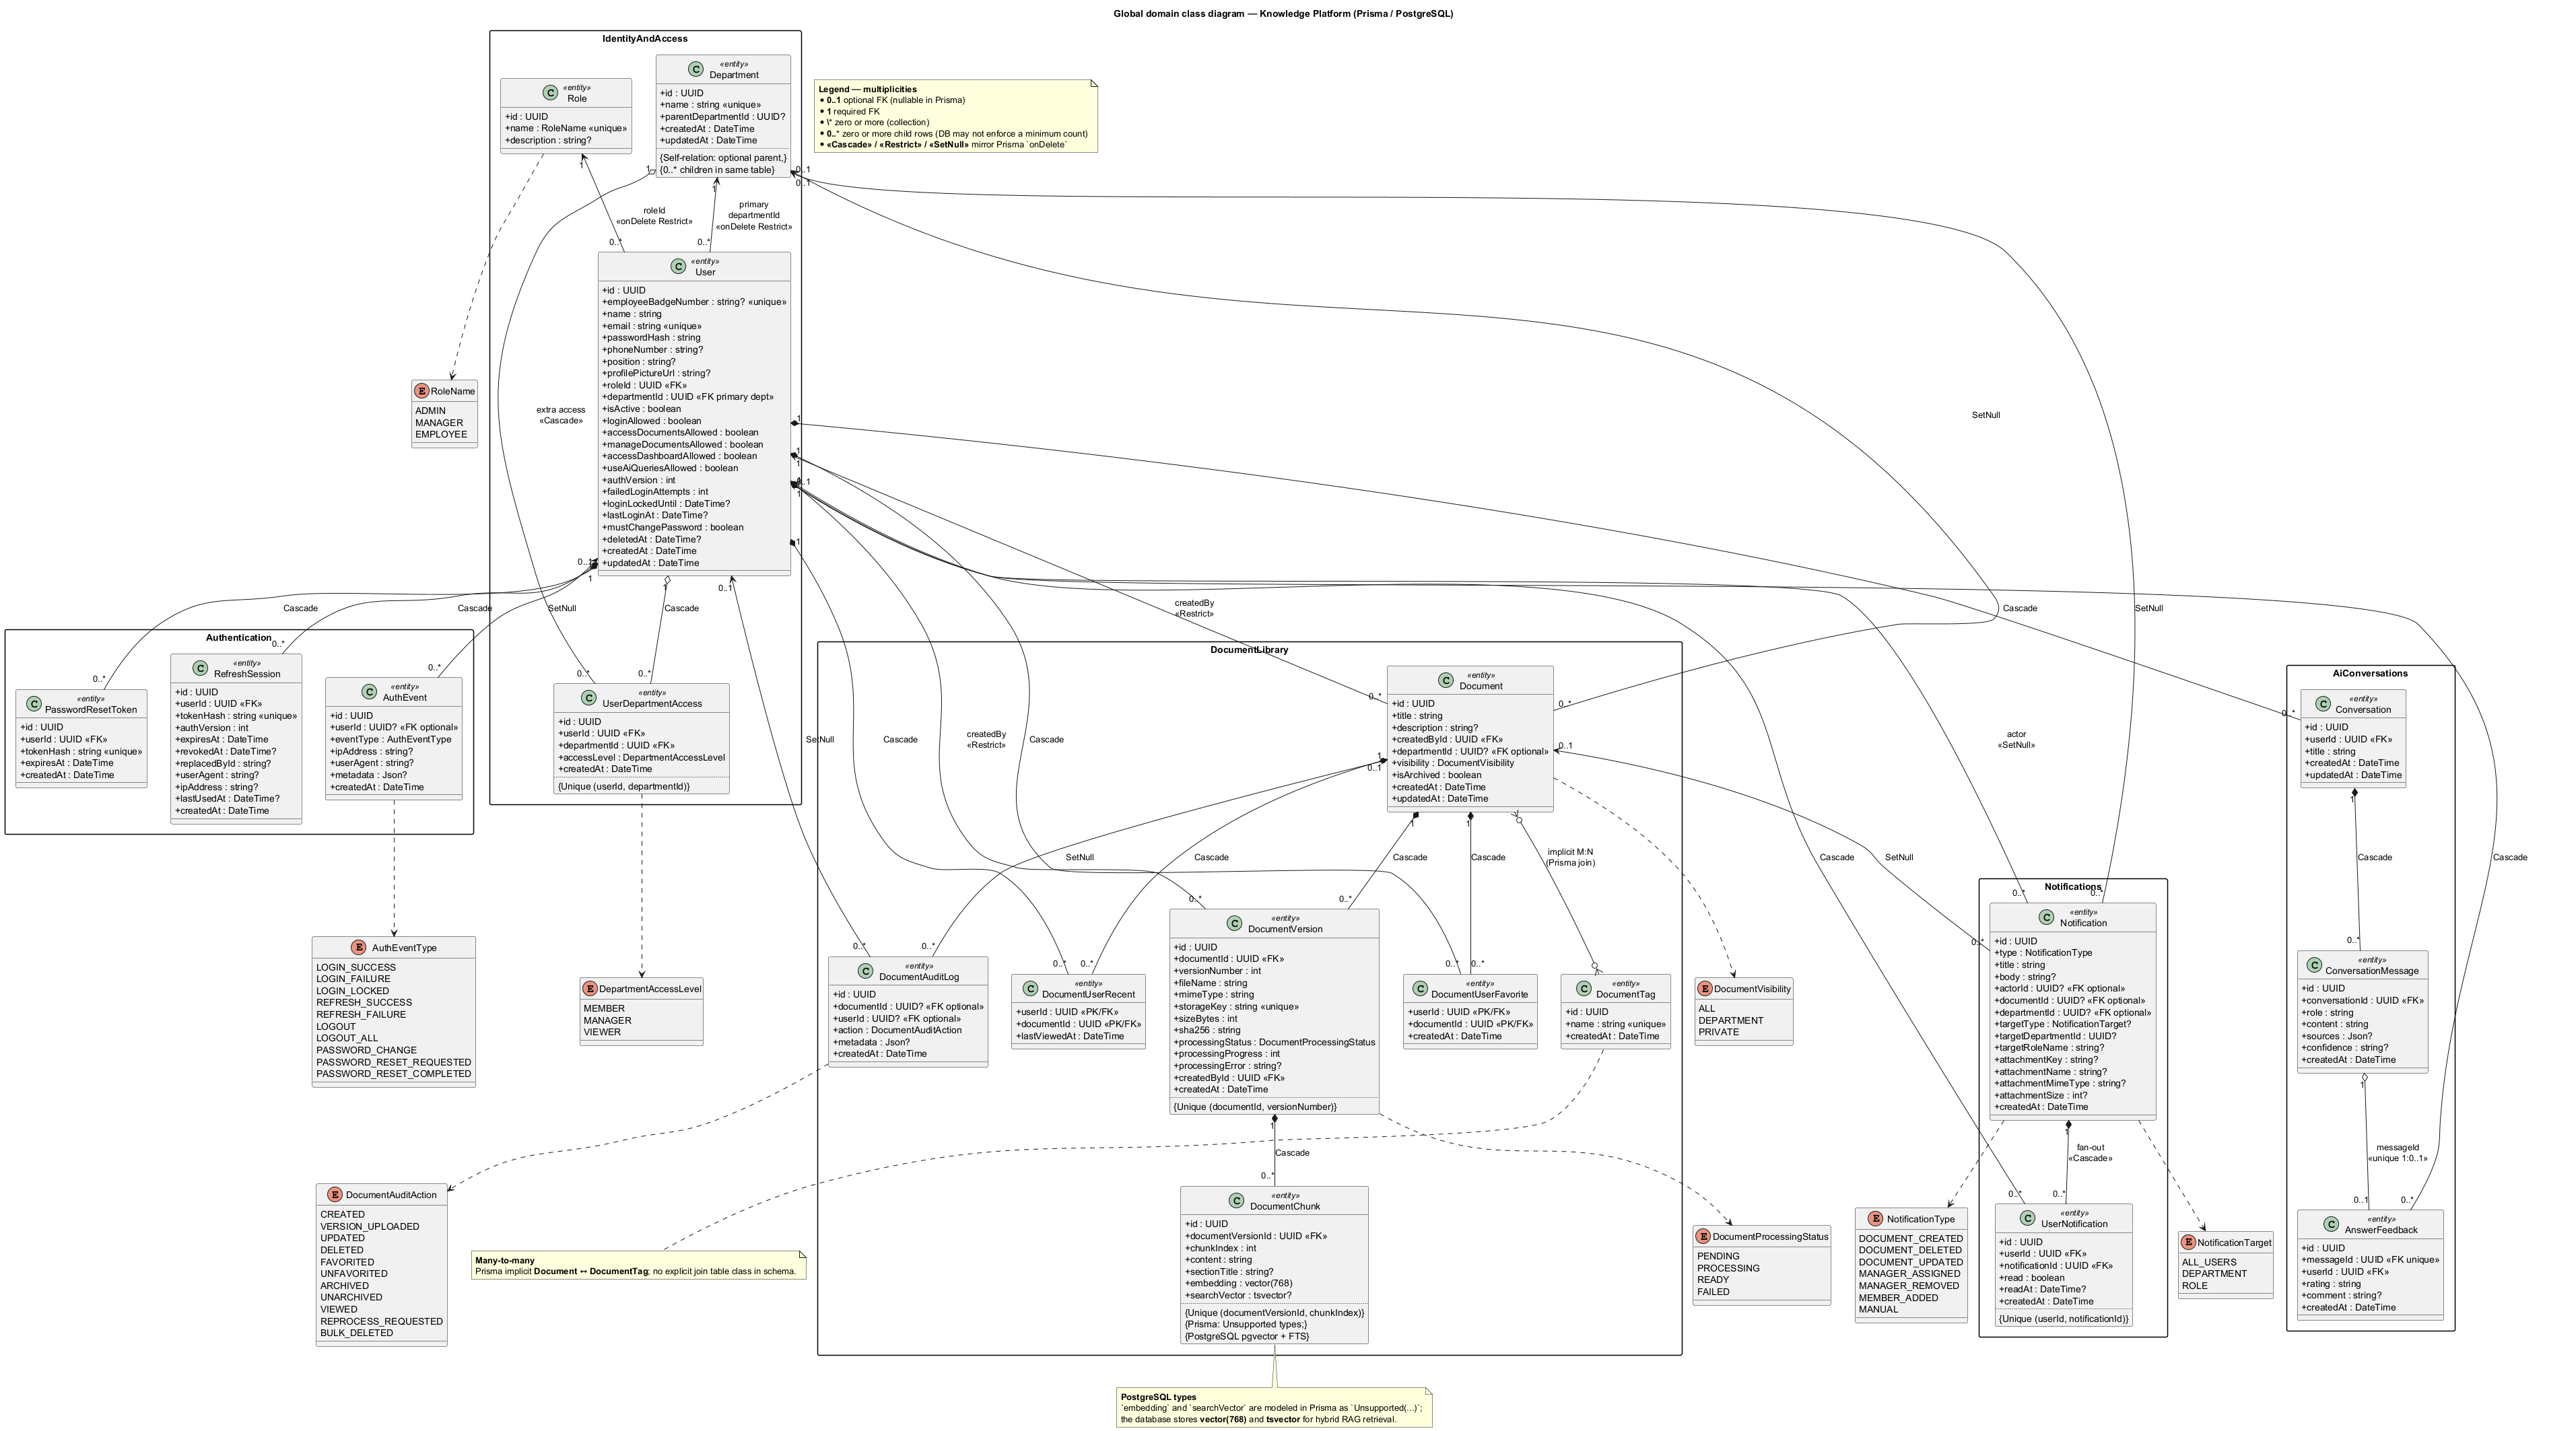
\includegraphics[width=0.98\textwidth,keepaspectratio]{assets/figures/global-class-knowledge-platform.png}
\caption{Global domain class diagram (persisted entities and main relationships)}
\label{fig:class-diagram}
\end{figure}

\section{Technology Choice Justification}
\label{sec:technology-justification}

Table~\ref{tab:decision-matrix} scores architectural options (1 = weak, 3 = strong).
The selected stack favours a TypeScript monorepo with Express and Next.js for
streaming RAG, operational simplicity, and alignment with project skills.

\begin{table}[H]
\centering
\caption{Decision-support matrix for platform architecture (scores: 1 = weak, 3 = strong)}
\label{tab:decision-matrix}
\renewcommand{\arraystretch}{1.4}
\setlength{\tabcolsep}{5pt}
\begin{tabularx}{\textwidth}{|>{\RaggedRight\arraybackslash}p{2.6cm}|>{\Centering\arraybackslash}p{1.7cm}|>{\Centering\arraybackslash}p{1.3cm}|>{\Centering\arraybackslash}p{2.1cm}|Y|}
\hline
\rowcolor{sectionblue!15}
\textbf{Criterion} &
\textbf{Monorepo} &
\textbf{Django} &
\textbf{Microservices} &
\textbf{Rationale} \\
\hline
Time to market & 3 & 2 & 1 & Shared TypeScript types; one repository \\
\hline
SSE streaming fit & 3 & 2 & 2 & Native Express streaming for RAG \\
\hline
Team skill alignment & 3 & 2 & 1 & Matches React + Node stack \\
\hline
Operational complexity & 3 & 3 & 1 & Single API process + worker \\
\hline
\end{tabularx}
\end{table}

\textbf{PostgreSQL + pgvector vs.\ dedicated vector DB:} colocating relational and vector data simplifies hybrid SQL+vector retrieval, transactional consistency, and department filters in one query layer~\cite{pgvector-docs}.

\textbf{Gemini vs.\ open-weight models:} the embedding and chat APIs reduce operational burden while providing strong multilingual embeddings (768 dimensions in this deployment)~\cite{google-gemini-docs}.

\textbf{In-process BullMQ worker vs.\ separate worker service:} embedding the consumer in the API process reduces deployment complexity for an academic/prototype-scale platform, at the cost of horizontal scaling coupling.

Table~\ref{tab:traceability-main} links representative requirements to the chosen
design elements and validation artefacts (see also Table~\ref{tab:fr-traceability}
in Chapter~\ref{ch:requirements}).

\begin{table}[H]
\centering
\caption{Requirements-to-design traceability (excerpt)}
\label{tab:traceability-main}
\footnotesize
\renewcommand{\arraystretch}{1.35}
\setlength{\tabcolsep}{4pt}
\begin{tabularx}{\textwidth}{|>{\RaggedRight\arraybackslash}p{1.0cm}|>{\RaggedRight\arraybackslash}p{2.5cm}|Y|>{\RaggedRight\arraybackslash}p{2.6cm}|}
\hline
\rowcolor{sectionblue!15}
\textbf{Req.} & \textbf{Design choice} & \textbf{Implemented element} & \textbf{Validation} \\
\hline
FR-01 & JWT + refresh rotation &
\tcodelines{auth.ts}{authClient.ts} &
\testfile{auth.integration.test} \\
\hline
FR-02 & Avatar CORP header &
\tcode{avatarsPublic.ts} &
\testfile{avatars.integration.test} \\
\hline
FR-03 & Async ingest queue &
\tcode{BullMQ + Redis} &
\testfile{documents.integration.test} \\
\hline
FR-07 & Hybrid RAG + SSE &
\tcodelines{search.ts}{ragCompletion.ts} &
\testfile{search.integration.test} \\
\hline
FR-10 & Admin RBAC &
\tcode{admin.ts} &
\testfile{admin.integration.test} \\
\hline
NFR-02 & Helmet + rate limits &
\tcode{httpApp.ts} &
manual + integration \\
\hline
\end{tabularx}
\end{table}

\section{Dynamic Interaction Design by Sprint}
\label{sec:sprint-design}

Sections~\ref{sec:overall-architecture}--\ref{sec:technology-justification} describe
\textbf{what} the platform is made of (components, data, and technology). This section
describes \textbf{how} actors and subsystems interact at runtime. For each sprint in
Table~\ref{tab:sprints} of Chapter~\ref{ch:requirements}, the design is organised in
three layers:
\begin{enumerate}[leftmargin=*,itemsep=0.2em]
  \item \textbf{Sprint scope} --- objectives and mapped functional requirements;
  \item \textbf{Scoped structural views} --- sprint use-case model and sprint domain class model;
  \item \textbf{Interaction sequence diagrams} --- request/response flows between client, API, workers, and external services.
\end{enumerate}
The full diagram catalog is indexed in Appendix~\ref{annex:diagrams}; implementation
evidence appears in Chapter~\ref{ch:implementation} and validation in
Chapter~\ref{ch:validation}.

\subsection{Sprint 1: Authentication and access control}\label{subsec:sprint1-design}

Sprint~1 establishes the security perimeter of the platform. It delivers
credential-based authentication with refresh-token rotation (FR-01), profile and
avatar management (FR-02), per-user feature restrictions (FR-12), and the
non-functional controls for HTTP hardening and single-flight token refresh
(NFR-02, NFR-03).

\sprintstructural{1}%
  {Sprint 1 use-case diagram — Authentication and access control}{fig:sprint1-use-cases}%
  {Sprint 1 domain class diagram — Authentication and access control}{fig:sprint1-class}

\sprintsequences{1}

\sprintflowgroup{Authentication and session management}

\paragraph{User login.}
The login flow validates email and password against bcrypt hashes, enforces account
lockout after repeated failures, and issues a short-lived access JWT together with
an HttpOnly refresh cookie bound to a token family stored in the database.
\seqdiagram{seq-01-login}{User login}{POST /auth/login}{fig:seq-01}

\paragraph{Access token refresh and session rotation.}
When the in-memory access token expires, the web client triggers a single
in-flight refresh request that rotates the refresh cookie, invalidates the
previous family member, and returns a new access token without user interaction.
\seqdiagram{seq-02-refresh-token}{Access token refresh and session rotation}{POST /auth/refresh}{fig:seq-02}

\paragraph{User logout.}
Logout revokes the active refresh-token family server-side and clears the
HttpOnly cookie, ensuring that stolen refresh tokens cannot be reused after the
user explicitly ends the session.
\seqdiagram{seq-03-logout}{User logout}{POST /auth/logout}{fig:seq-03}

\paragraph{Forgot and reset password.}
Password recovery sends a time-limited reset link by email; the reset endpoint
validates the token, applies the password policy, and invalidates all outstanding
refresh families for the affected account.
\seqdiagram{seq-04-password-reset}{Forgot and reset password}{POST /auth/forgot-password, reset-password}{fig:seq-04}

\paragraph{Change password with session invalidation.}
Authenticated users may change their password by supplying the current secret;
successful rotation updates the hash, enforces policy rules, and terminates other
active sessions through family revocation.
\seqdiagram{seq-05-change-password}{Change password with session invalidation}{POST /auth/change-password}{fig:seq-05}

\sprintflowgroup{Profile, restrictions and session context}

\paragraph{Profile update.}
Profile updates accept display name and avatar file uploads; the API persists
metadata in Prisma and stores avatar binaries on disk, exposing them through the
public \texttt{/avatars} route with cross-origin headers.
\seqdiagram{seq-06-profile-update}{Profile update}{PATCH /auth/profile}{fig:seq-06}

\paragraph{Feature restriction enforcement.}
Middleware consults per-user feature flags before protected handlers execute;
restricted users receive a structured \texttt{403 FEATURE\_RESTRICTED} response
that the web client maps to a dedicated explanation page.
\seqdiagram{seq-07-feature-restriction}{Feature restriction enforcement}{403 FEATURE\_RESTRICTED}{fig:seq-07}

\paragraph{Current user session payload.}
The \texttt{/me} endpoint returns the authenticated principal, role, department
memberships, and active feature restrictions so the client can render navigation
and gate UI affordances without additional round trips.
\seqdiagram{seq-23-get-auth-me}{Current user session payload}{GET /auth/me}{fig:seq-23}

\sprintflowgroup{Guest and restricted UX pages}

\paragraph{Register information page (no self-service signup).}
Self-service registration is intentionally disabled; the static \texttt{/register}
page informs visitors that accounts are provisioned by administrators, avoiding
orphan users outside the RBAC model.
\seqdiagram{seq-32-register-info-static}{Register information page (no self-service signup)}{Next.js /register}{fig:seq-32}

\paragraph{Restricted feature explanation page.}
When the API signals a feature restriction, the client redirects to
\texttt{/restricted}, presenting context-sensitive guidance rather than a generic
error banner.
\seqdiagram{seq-33-restricted-page-ux}{Restricted feature explanation page}{/restricted UX}{fig:seq-33}

\subsection{Sprint 2: Document library and ingest}\label{subsec:sprint2-design}

Sprint~2 implements the document corpus lifecycle: multi-format upload and storage
(FR-03), department-scoped visibility enforcement (FR-04), and library
organisation features such as versioning, tags, favorites, and recents (FR-05).
Uploads are accepted synchronously by the API while text extraction, chunking, and
embedding run asynchronously in a BullMQ worker.

\sprintstructural{2}%
  {Sprint 2 use-case diagram — Document library and ingest}{fig:sprint2-use-cases}%
  {Sprint 2 domain class diagram — Document library and ingest}{fig:sprint2-class}

\sprintsequences{2}

\sprintflowgroup{Upload and asynchronous ingest}

\paragraph{Document upload.}
The upload endpoint validates MIME type and size, writes the binary to disk,
creates \texttt{Document} and \texttt{DocumentVersion} rows, and enqueues an
ingest job keyed by version identifier.
\seqdiagram{seq-08-document-upload}{Document upload}{POST /documents/upload}{fig:seq-08}

\paragraph{Asynchronous ingest worker.}
The BullMQ consumer loads the stored file, extracts text per format, splits
content into sentence-aware chunks with table preservation, computes
768-dimensional embeddings, and persists \texttt{Chunk} rows indexed for retrieval.
\seqdiagram{seq-09-document-ingest-worker}{Asynchronous ingest worker}{BullMQ processIngest}{fig:seq-09}

\paragraph{Reprocess document version.}
Administrators can force re-ingestion of an existing version---for example after
embedding model upgrades---without re-uploading the binary.
\seqdiagram{seq-29-document-reprocess}{Reprocess document version}{POST .../reprocess}{fig:seq-29}

\sprintflowgroup{Library access and download}

\paragraph{Document file download.}
Authorized users download the original file through a version-scoped endpoint that
re-checks department visibility before streaming bytes from the storage backend.
\seqdiagram{seq-10-document-read-download}{Document file download}{GET .../file}{fig:seq-10}

\paragraph{Document list.}
The list endpoint applies department filters, search facets, and pagination,
returning summary metadata suitable for the library grid without loading chunk
payloads.
\seqdiagram{seq-24-documents-list}{Document list}{GET /documents}{fig:seq-24}

\paragraph{Document detail.}
Detail retrieval joins document metadata, active version, tags, ingest status, and
audit hints, giving the preview pane everything required for inline viewing.
\seqdiagram{seq-25-document-detail}{Document detail}{GET /documents/:id}{fig:seq-25}

\paragraph{Favorites and recents.}
Users pin documents to favorites and the API records recent views; both features
are scoped to the authenticated principal and surfaced on the library home view.
\seqdiagram{seq-26-favorites-recents}{Favorites and recents}{POST/DELETE favorite, recent view}{fig:seq-26}

\sprintflowgroup{Metadata and versioning}

\paragraph{Document metadata update.}
Managers and owners may patch title, description, tags, and visibility; changes
are validated against writable department scopes and written to the audit trail.
\seqdiagram{seq-27-patch-document-metadata}{Document metadata update}{PATCH /documents/:id}{fig:seq-27}

\paragraph{New document version.}
Uploading a replacement file creates a new \texttt{DocumentVersion}, triggers a
fresh ingest job, and keeps prior versions available for rollback and audit.
\seqdiagram{seq-28-document-new-version}{New document version}{POST /documents/:id/versions}{fig:seq-28}

\subsection{Sprint 3: Search, RAG and conversations}\label{subsec:sprint3-design}

Sprint~3 delivers the intelligent retrieval layer: semantic search over embedded
chunks (FR-06), hybrid retrieval-augmented generation with streaming answers
(FR-07), and persistent conversation threads with feedback (FR-08). The RAG
evaluation harness (NFR-06) is introduced in parallel to measure answer quality
against golden datasets.

\sprintstructural{3}%
  {Sprint 3 use-case diagram — Search, RAG and conversations}{fig:sprint3-use-cases}%
  {Sprint 3 domain class diagram — Search, RAG and conversations}{fig:sprint3-class}

\sprintsequences{3}

\sprintflowgroup{Search and hybrid RAG}

\paragraph{Semantic vector search.}
The semantic search endpoint embeds the user query, queries pgvector with
department filters, and returns ranked chunks with snippet previews for quick
exploration outside the chat UI.
\seqdiagram{seq-11-semantic-search}{Semantic vector search}{POST /search/semantic}{fig:seq-11}

\paragraph{Hybrid RAG Ask with SSE streaming.}
The Ask endpoint orchestrates query optimisation, dense and sparse retrieval,
reciprocal-rank fusion, LLM reranking, and streams tokens plus source citations
to the browser over Server-Sent Events.
\seqdiagram{seq-12-ask-rag-sse}{Hybrid RAG Ask with SSE streaming}{POST /search/ask}{fig:seq-12}

\sprintflowgroup{Conversations and answer quality}

\paragraph{Conversation and messages.}
Users create conversation threads, append questions, and retrieve message history;
each assistant turn stores retrieved sources, confidence metadata, and links back
to originating chunks.
\seqdiagram{seq-13-conversation-and-messages}{Conversation and messages}{/conversations}{fig:seq-13}

\paragraph{Answer feedback.}
After each answer, users may submit thumbs-up/down feedback with optional comments;
the API persists \texttt{AnswerFeedback} rows used later for quality dashboards.
\seqdiagram{seq-14-answer-feedback}{Answer feedback}{POST .../feedback}{fig:seq-14}

\paragraph{Conversation CRUD supplement.}
Beyond the primary messaging flow, clients list, rename, and delete conversations
through supplementary endpoints that keep thread metadata consistent with UI state.
\seqdiagram{seq-30-conversations-crud-supplement}{Conversation CRUD supplement}{list, patch, delete}{fig:seq-30}

\paragraph{Admin feedback statistics.}
Administrators query aggregated feedback metrics---volume, sentiment ratio, and
recent comments---to monitor RAG quality trends across departments.
\seqdiagram{seq-31-admin-feedback-stats}{Admin feedback statistics}{GET /conversations/feedback/stats}{fig:seq-31}

\subsection{Sprint 4: Governance and notifications}\label{subsec:sprint4-design}

Sprint~4 covers organisational governance: automatic and manual notifications
(FR-09), administrator tooling for users, departments, and bulk operations
(FR-10), and the manager department dashboard (FR-11). Notification events are
decoupled from document mutations through a service layer, while admin routes
enforce elevated RBAC and emit structured audit records for every destructive
action.

\sprintstructural{4}%
  {Sprint 4 use-case diagram — Governance and notifications}{fig:sprint4-use-cases}%
  {Sprint 4 domain class diagram — Governance and notifications}{fig:sprint4-class}

\sprintsequences{4}

\sprintflowgroup{Notification subsystem}

\paragraph{Automatic notification on document events.}
When documents are created or materially updated, the notification service fans
out inbox entries to subscribed department members without blocking the upload
response path.
\seqdiagram{seq-15-notification-automatic}{Automatic notification on document events}{notifyDocumentCreated}{fig:seq-15}

\paragraph{Manual announcement.}
Administrators compose announcements with optional attachments; the send endpoint
validates audience scope and delivers messages to targeted user inboxes.
\seqdiagram{seq-16-notification-manual-send}{Manual announcement}{POST /notifications/send}{fig:seq-16}

\paragraph{Notification inbox.}
Users list notifications, query unread counts, mark items as read, and download
attachments through REST endpoints polled by the web shell.
\seqdiagram{seq-17-notification-inbox}{Notification inbox}{list, unread, mark read, attachment}{fig:seq-17}

\sprintflowgroup{Manager dashboard}

\paragraph{Manager department overview.}
Managers retrieve department-scoped KPIs---document counts, recent activity, and
team membership---through dedicated \texttt{/manager} routes filtered to
manageable departments.
\seqdiagram{seq-18-manager-dashboard}{Manager department overview}{GET /manager/*}{fig:seq-18}

\sprintflowgroup{Administrator governance}

\paragraph{Admin create user.}
Administrators provision accounts with initial roles, department assignments, and
optional feature restrictions; credentials are communicated out-of-band per
organisational policy.
\seqdiagram{seq-19-admin-user-create}{Admin create user}{POST /admin/users}{fig:seq-19}

\paragraph{Admin merge departments.}
Department merge consolidates documents, access grants, and memberships from a
source department into a target, preserving referential integrity inside a
transaction.
\seqdiagram{seq-20-admin-department-merge}{Admin merge departments}{POST /admin/departments/merge}{fig:seq-20}

\paragraph{Bulk department access.}
Bulk PUT replaces the full access matrix for a user or department in one request,
simplifying onboarding scripts and CSV-driven imports.
\seqdiagram{seq-21-admin-department-access-bulk}{Bulk department access}{PUT .../department-access}{fig:seq-21}

\paragraph{Admin create department.}
New organisational units are created with unique slugs; the operation is restricted
to administrators and is logged for compliance review.
\seqdiagram{seq-34-admin-department-create}{Admin create department}{POST /admin/departments}{fig:seq-34}

\paragraph{Single department access grant/revoke.}
Fine-grained POST and DELETE endpoints add or remove individual department access
rows without rewriting the entire access matrix.
\seqdiagram{seq-35-dept-access-single-post-delete}{Single department access grant/revoke}{POST/DELETE access}{fig:seq-35}

\paragraph{Admin KPI statistics.}
The admin statistics endpoint aggregates platform-wide counters---users,
documents, conversations, and ingest backlog---for dashboard cards.
\seqdiagram{seq-36-admin-stats}{Admin KPI statistics}{GET /admin/stats}{fig:seq-36}

\paragraph{Admin activity log and CSV export.}
Administrators browse paginated activity logs and export filtered events to CSV for
offline analysis, with formula-injection escaping on downloadable fields.
\seqdiagram{seq-37-admin-activity-export}{Admin activity log and CSV export}{GET /admin/activity}{fig:seq-37}

\paragraph{Document audit trail.}
Per-document audit views expose who changed metadata, visibility, or versions,
supporting forensic review during access reviews.
\seqdiagram{seq-38-admin-document-audit}{Document audit trail}{GET /admin/document-audit}{fig:seq-38}

\paragraph{Documents CSV export.}
Administrators export the document catalogue---titles, departments, tags, and ingest
status---as CSV for inventory reconciliation.
\seqdiagram{seq-39-admin-documents-csv-export}{Documents CSV export}{GET /documents/export}{fig:seq-39}

\paragraph{Bulk document delete.}
Bulk delete accepts a list of document identifiers, verifies administrator scope,
removes storage artefacts, and cascades database rows inside a guarded transaction.
\seqdiagram{seq-40-admin-bulk-delete-documents}{Bulk document delete}{POST /documents/bulk-delete}{fig:seq-40}

\paragraph{Admin user patch and lock.}
Administrators update user roles, restrictions, and lock state; account lock
immediately invalidates refresh families to block further API access.
\seqdiagram{seq-41-admin-user-patch-lock}{Admin user patch and lock}{PATCH/lock user}{fig:seq-41}

\subsection{Sprint 5: Operations, testing and deployment}\label{subsec:sprint5-design}

Sprint~5 hardens operability and reproducibility: a public health probe (NFR-01),
containerised deployment (NFR-04), a broad integration-test suite (NFR-05), and
the RAG evaluation harness (NFR-06). Unlike feature sprints, several deliverables
are cross-cutting quality gates rather than user-visible flows.

\sprintstructural{5}%
  {Sprint 5 use-case diagram — Operations, testing and deployment}{fig:sprint5-use-cases}%
  {Sprint 5 domain class diagram — Operations, testing and deployment}{fig:sprint5-class}

\sprintsequences{5}

\paragraph{API health probe.}
Load balancers and orchestrators call \texttt{GET /health} to verify that the API
process is running and can reach PostgreSQL and Redis; the endpoint returns a
compact JSON status without authentication.
\seqdiagram{seq-22-health-check}{API health probe}{GET /health}{fig:seq-22}

\subsubsection{Operational deliverables}
\label{subsubsec:sprint5-operations}

\paragraph{Integration test suite.}
The API ships with a Vitest and Supertest integration suite spanning
authentication, documents, search, conversations, admin, and manager routers.
Tests spin up an isolated database schema, seed fixtures, and assert HTTP
contracts against the same routes documented in the sequence diagrams above,
providing regression coverage for NFR-05.

\paragraph{Docker Compose deployment.}
Production-oriented Compose files package the API, web, PostgreSQL with pgvector,
and Redis behind documented environment variables and volume mounts. Migrations run
through the Prisma CLI inside the API container, ensuring that any workstation
or CI agent can reproduce the full stack with a single \texttt{docker compose up}
invocation (NFR-04).

\paragraph{RAG evaluation harness.}
A command-line evaluation harness loads golden question--answer pairs, invokes the
Ask pipeline programmatically, and scores responses with an automated LLM judge.
Reports are written to \texttt{eval-reports/} so retrieval prompt changes can be
compared across commits, fulfilling the reproducible quality gate of NFR-06.


\section{Chapter Conclusion}

This chapter defined the architectural foundation of the Knowledge Platform in two
complementary views: static design (architecture, subsystems, domain model, and
technology justification) and dynamic design (sprint-scoped structural views and
interaction sequence diagrams). The decision matrix and requirements-to-design
traceability established that each major functional and non-functional requirement
is mapped to concrete modules, interaction flows, and validation evidence.
Chapter~\ref{ch:implementation} describes how these design artefacts were realized
in code.
